\documentclass[12pt]{beamer}
\usetheme{CambridgeUS}
\usepackage[utf8]{inputenc}
\usepackage[spanish]{babel}
\usepackage{amsmath}
\usepackage{amsfonts}
\usepackage{amssymb}
\usepackage{graphicx}

\author{Kevin Steven García \\ Cesar Andres Saavedra}
\title{Generación de números aleatorios \\ Modelos probabilisticos \\ Pruebas de bondad de ajuste}
%\setbeamercovered{transparent} 
%\setbeamertemplate{navigation symbols}{} 
%\logo{} 
\institute{Universdiad del Valle \\ Estadística \\ Simulación Estadística} 
\subject{} 
\date{Abril 2018}


\begin{document}

\begin{frame}
\titlepage
\end{frame}


\begin{frame}
\frametitle{Introducción}

\begin{block}{\textbf{Distribucion Poisson:} 
~\\La distribución de Poisson es, una de las mas importantes distribuciones de probabilidad discretas, es decir, aquellas de las cuales pueden tomar los valores 0,1,2,3,...,k.  
~\\Cada una de las Variables aleatorias representa el numero total de ocurrencias de un fenómeno durante un periodo de tiempo fijo o en una región fija del espacio y expresa la probabilidad de un numero k de ocurrencias.}
\end{block}
\end{frame}

\begin{frame}
\begin{block}{\textbf{Distribucion Logistica:}
~\\La distribución Logística es una distribución de probabilidad continua cuya función de distribución es la función logística, que aparece en el contexto de la regresión logística. Siendo la regresión logística un instrumento estadístico de análisis multivariado, de uso explicativo y predictivo. Que resulta útil cuando se tiene una variable dependiente dicotomica, atributo de ausencia o presencia que se puntuá con valores de 1 y 0, respectivamente.}
\end{block} 
\end{frame}

\begin{frame}
\frametitle{ Artículos}
\begin{itemize}
\begin{block}{\item\textbf{Evidence in support of seismic hazard following Poisson distribution.\\Pruebas de apoyo al riesgo sísmico tras la distribución Poisson.}}
\end{block} 
\end{itemize}

\begin{itemize}
\begin{block}{\item\textbf{APLICAÇÃO DE REGRESSÃO LOGÍSTICA E ALGORITMOS GENÉTICOS NA ANÁLISE DE RISCO DE CRÉDITO.\\Aplicación de la regresión logística y de los algoritmos genéticos en el análisis del riesgo de crédito.}}
\end{block} 
\end{itemize}
\end{frame}

\begin{frame}
\frametitle{Simulación Distribuciones }
\begin{figure}
\centering
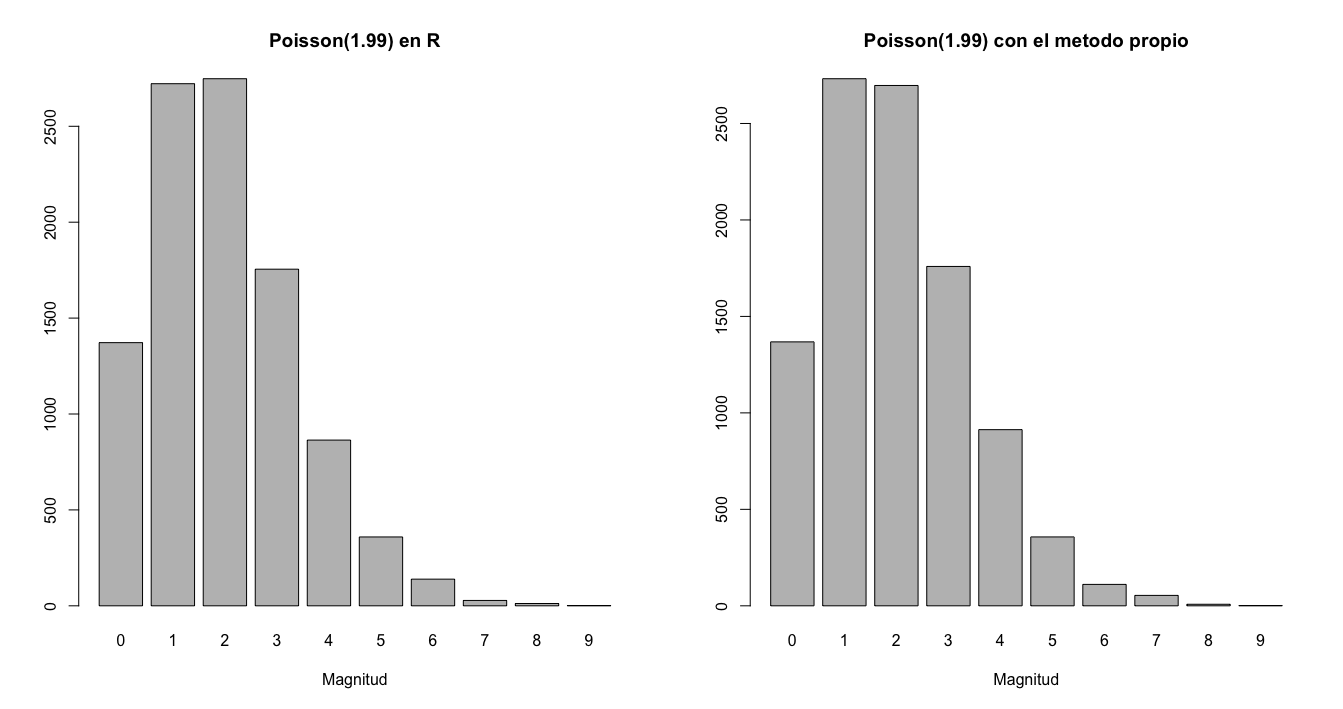
\includegraphics[scale=0.3]{imagenes/Rplot1.png}
\caption{Comparación simulaciones en R y con el método propio de la distribución Poisson($\lambda=1.99$)}\label{figura2}
\end{figure}
\end{frame}

\begin{frame}
\frametitle{Simulación Distribuciones}
\begin{figure}
\centering
\includegraphics[scale=0.3]{imagenes/logic.png}
\caption{Comparación simulaciones en R y con el método de la transformada inversa para la distribución Logistica($a=0,b=2$)}\label{figura2}
\end{figure}
\end{frame}

\begin{frame}
\frametitle{Simulación Pruebas de bondad de ajuste}
\begin{figure}
\centering
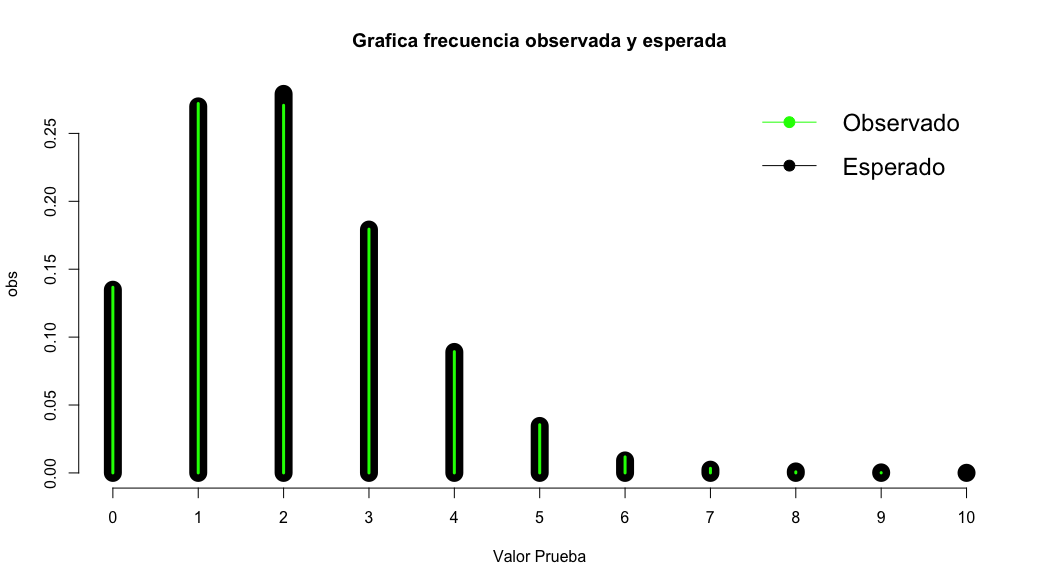
\includegraphics[scale=0.3]{imagenes/poisson.png}
\caption{Frecuencia esperada y observada Poisson $(\lambda=1.99)$}\label{figura2}
\end{figure}
\end{frame}

\begin{frame}
\frametitle{Simulación Pruebas de bondad de ajuste}
\begin{tabular}{cccc}
\hline 
OBSERVACIÓN & OBS & ESP & $(OBS-ESP)^2/ESP$ \\  
0 & 0.1404 & 0.1367 & 0.000100 \\  
1 & 0.2733 & 0.2720 & 0.000006 \\  
2 & 0.2617 & 0.2706 & 0.000292 \\  
3 & 0.1761 & 0.1795 & 0.000064 \\  
4 & 0.0933 & 0.0893 & 0.000179 \\ 
5 & 0.0390 & 0.0355 & 0.000345 \\  
6 & 0.0125 & 0.0118 & 0.000041 \\  
7 & 0.0033 & 0.0033 & 0 \\  
8 & 0.0002 & 0.0008 & 0.00045 \\  
9 & 0.0002 & 0.0001 & 0.0001 \\ 
\hline 
\end{tabular} 
~\\ El estadístico de prueba de la prueba $\chi^2$ de Pearson nos dio $\chi_{obs}^{2}=\sum\limits_{i=1}^{k}\frac{(O_{i}-E_{i})^2}{E_{i}}=0.0015792$  
~\\ El $p-valor=P(\chi^{2}_{k-m-1}>\chi^{2}_{obs})=P(\chi^{2}_{8}>0.0015792)=1$.
\end{frame}

\begin{frame}
\frametitle{Simulación Pruebas de bondad de ajuste}
\begin{figure}
  \centering
  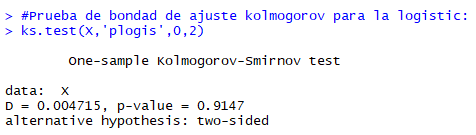
\includegraphics[scale=0.5]{imagenes/k.png}
  \caption{Resultados prueba de Kolmogorov para los valores generados con el método de la transformada inversa para la Logistic($a=0,b=2$)}\label{figura1}
\end{figure}
\end{frame}

%\begin{frame}
%\frametitle{Resultados}
%\end{frame}

\begin{frame}
\frametitle{Conclusiones}
\begin{itemize}
\item Se puede concluir que estas distribuciones tienen un uso muy importante en problemas sociales y económicos de gran tamaño. Por un lado, la distribución Poisson se utilizó para tratar de modelar y mitigar el riesgo sísmico (completar conclusión del articulo). Por otro lado, la distribución Logistic se usó para predecir u obtener la probabilidad por medio de un modelo logit, de que un cliente sea buen o mal pagador en cuanto a sus créditos personales dadas ciertas características, esto es muy importante en las empresas financieras, ya que con tan solo unas pocas preguntas personales al cliente, pueden obtener dicha probabilidad logrando disminuir considerablemente los riesgos crediticios, evitando así generar inmensas perdidas en la empresa.
\end{itemize}
\end{frame}

\begin{frame}
\frametitle{Conclusiones}
\begin{itemize}
\item Con respecto a los métodos de simulación y pruebas de bondad de ajuste utilizadas, podemos ver que tanto el método utilizado para la distribución Poisson (método propio) como para la Logística (método de la transformada inversa) son muy acertados como generadores de variables aleatorias, ya que generan casi identicamente datos que siguen dichas distribuciones, y esto se ve apoyado con las pruebas de bondad de ajuste utilizadas, ya que ambas se nos rechazan por mucho, es decir, los datos generados muestran demasiada evidencia de que siguen las distribuciones hipotéticas.
\end{itemize}
\end{frame}

\begin{frame}
\frametitle{Bibliografía}
\begin{block}{\textbf {Statistical distributions, Catherine Forbes, Merran Evans, Nicholas Hastings, Brian Peacock, Fourth edition.}}
\end{block}	
\begin{block}{\textbf {http://www.redalyc.org/html/750/75040605/}}
\end{block}
\begin{block}{\textbf {https://www.sciencedirect.com.bd.univalle.edu.co}}
\end{block}
\end{frame}

\end{document}